% $Id$
% ..............................................................................
%                V E R S C H L U E S S E L U N G S V E R F A H R E N
%
% Writing rule: Capitel header with all nouns/verbs-words capitalized,
%               All other headers in the normal lower/upper case manner
%               like sentences (without a dot at the end).
% Writing rule: Use American English instead of British English consistently.
%
% ~~~~~~~~~~~~~~~~~~~~~~~~~~~~~~~~~~~~~~~~~~~~~~~~~~~~~~~~~~~~~~~~~~~~~~~~~~~~~~
%------------------------------------------------------------------------------
% First Editor: Christine St�tzel, April 2004
% Update and corrections: B. Esslinger, June 2005
% Update and corrections: B. Esslinger, June 2005
% Update B. Esslinger and Minh Van Nguyen, July 2009 
%------------------------------------------------------------------------------

% ``primenet''
\newpage
\hypertarget{Kapitel_PaperandPencil}{}

\chapter{Paper and Pencil Encryption Methods}
\label{Kapitel_PaperandPencil}
(Christine St\"otzel, April 2004; Updates: B.+C. Esslinger, June 2005; Updates Minh Van Nguyen and B. Esslinger, July 2009)
\index{Paper- and pencil methods}

\begin{center}
\fbox{\parbox{15cm}{%
{\em Edgar Allan Poe\index{Poe, Edgar Allan}: 
A Few Words on Secret Writing, 1841}\\
Few persons can be made to believe that it is not quite an easy thing
to invent a method of secret writing which shall baffle investigation.
Yet it may be roundly asserted that human ingenuity cannot concoct a
cipher which human ingenuity cannot resolve.}}
\end{center}

The following chapter provides a broad overview of paper and pencil 
methods\footnote{%
The footnotes to this chapter describe how the methods can be
performd using CrypTool CrypTool 1.
Additionally the last sub chapter (\ref{PaP_Sage_samples})
contains example code using the computer algebra system Sage\index{Sage}.
                 }
each with references to deeper information.
All techniques that people can apply manually to en- and decipher a message are 
embraced by this term. These methods were and still are especially popular with
secret services, as a writing pad and a pencil -- in contrast to electronic
aids -- are totally unsuspicious.

The first paper- and pencil methods already arose about 3000 years ago, but new
procedures were developed during the past century, too. All paper and pencil 
methods are a matter of symmetric methods\index{Encryption!symmetric}. 
Even the earliest encryption algorithms use the basic principles such as 
transposition, substitution, block construction and their combinations. 
Hence it is worthwhile to closely consider this ``ancient'' methods especially
under didactic aspects.

Methods to be successful and wide-spread had to fulfill some attributes which are equally required for modern algorithms:
\begin{itemize}
\item Exhaustive description, almost standardization (including special cases,
      padding, etc.).
\item Good balance between security and usability 
      (because methods being too complicated were error-prone or
      unacceptably slow).
\end{itemize}


\newpage
%------------------------------------------------------------------------------
\section{Transposition ciphers}
\label{PaP_transposition_ciphers}
\index{Transposition}

Encrypting a message by means of transposition\index{Transposition} does not 
change the original characters of this message, only their order is modified
(transposition = exchange)\footnote{Another name used for transposition is
permutation\index{Permutation}.}.

%------------------------------------------------------------------------------
\subsection{Introductory samples of different transposition ciphers}
\label{introsamplesTranspositionCiphers}

\begin{itemize}

\item {\bf Rail Fence}\footnote{%
   This method can directly be found in CrypTool\index{CrypTool} at the menu item
   {\bf Crypt/Decrypt \textbackslash{} Symmetric (classic) \textbackslash{} Scytale / Rail Fence}.
   You can simulate this method also under the menu {\bf Crypt/Decrypt \textbackslash{} 
   Symmetric (classic) \textbackslash{} Permutation}: For a Rail Fence with
   2 lines use as key ``B,A'' and accept the default settings (only one
   permutation, where your input is done line-by-line and the output is
   taken column-by-column). 
   Using the key ``A,B'' would start the zigzag pattern below in the
   way, that the first letter is written into the first line instead of the
   second line.}
   \cite{pp:Singh2001}\index{Rail Fence cipher}:
   The characters of a message are alternately written in two (or more) lines,
   creating a zigzag pattern. The resulting ciphertext is read out 
   line by line.\\
   This is more a children's method.

   Plaintext\footnote{If the alphabet only uses 26 letters, we write the
   plaintext in small letters and the ciphertext in capital letters.}%
   : an example of transposition

\begin{table}[ht]
\begin{center}
\begin{tabular}{r@{\:}r@{\:}r@{\:}r@{\:}r@{\:}r@{\:}r@{\:}r@{\:}r@{\:}r@{\:}r@{\:}r@{\:}r@{\:}r@{\:}r@{\:}r@{\:}r@{\:}r@{\:}r@{\:}r@{\:}r@{\:}r@{\:}r@{\:}r@{\:}}
	  & n &   & x &   & m &   & l &   & o &   & t &   & a &   & s &   & o &   & i &   & i &   & n \\
	a &   & e &   & a &   & p &   & e &   & f &   & r &   & n &   & p &   & s &   & t &   & o &   \\
\end{tabular}
\caption{Rail Fence cipher}
\end{center} 
\end{table}

   Ciphertext\footnote{The letters of the cleartext are -- as used 
   historically -- grouped within blocks of 5 letters. It does not matter
   if the (constant) block length is different or no blank is inserted.}%
   : NXMLO TASOI INAEA PEFRN PSTO\\


\item {\bf Scytale}\footnote{%
   This method can directly be found in CrypTool\index{CrypTool} at the menu item
   {\bf Crypt/Decrypt \textbackslash{} Symmetric (classic) \textbackslash{} Scytale / Rail Fence}.
   As this method is a special case of a simple columnar transposition, you also can
   simulate it in CrypTool\index{CrypTool} under the 
   menu {\bf Crypt/Decrypt \textbackslash{} Symmetric (classic) \textbackslash{} 
   Permutation}: For the Scytale within the dialog box only the first 
   permutation is used. If the wood has e.g. 4 angles use as key ``1,2,3,4''.
   This is equivalent to write the text horizontally in blocks of 4 letters 
   in a matrix and to read it out vertically . 
   Because the key is in an in ascending order, the Scytale is denoted as
   an identical permutation. And because writing and read-out is done only
   once it is a simple (and no double) permutation.}
   \cite{pp:Singh2001}\index{Scytale}%
   : 
   This method was probably used since 600 B.C. -- a description
   of how it operated is not known from before Plutarch (50-120 B.C.).\\
   A long strip of paper is wrapped around a wooden cylinder and then the 
   message is written along the length of this strip. The ciphertext is 
   produced by unwinding the strip.

\item {\bf Grille} \cite{pp:Goebel2003}: Both parties use identical stencils. 
   Line by line, their holes are filled with plaintext that is read out 
   column by column to produce the ciphertext. If there is plaintext left, 
   the procedure is repeated\footnote{%
   This method cannot be simulated with a pure column transposition.}.

   \hypertarget{turning-grille}{}
\item {\bf Turning grille} \cite{pp:Savard1999}%
   \index{Turning grille}: 
   The German army used turning 
   grilles during WW1\footnote{The turning grille was already invented in 
   1881 by Eduard Fleissner von Wostrowitz.\\
   A good visualization can be found under www.turning-grille.com.}%
   . 
   A square grille serves as a stencil, a quarter of its fields being holes.
   The first part of the message is written on a piece of paper through	these
   holes, then the grille is rotated by 90 degrees and the user can
   write down the second part of the message, etc. But this method does only
   work, if the holes are chosen carefully: Every field has to be used, and
   no field may be used twice, either. The ciphertext is read out line by
   line.

   In the example for a turning grille in the following table you can write
   4 times 16 characters of the cleartext on a piece of paper:
\begin{table}[ht]
\begin{center}
\begin{tabular}{|cccc|cccc|}
\hline 	
	O & - & - & - & - & O & - & - \\
	- & - & - & O & O & - & - & O \\
	- & - & - & O & - & - & O & - \\
	- & - & O & - & - & - & - & - \\
\hline 	
	- & - & - & - & O & - & - & - \\
	O & - & O & - & - & - & O & - \\
	- & O & - & - & - & - & - & O \\
	- & - & - & O & O & - & - & - \\
\hline
\end{tabular}  
\caption{8x8 turning grille} 
\end{center}   
\end{table}

\end{itemize}


%------------------------------------------------------------------------------
% {\bf Column and row transposition}
\subsection[Column and row transposition ciphers]
    {Column and row transposition\footnotemark}
    \footnotetext{%
Most of the following methods can be simulated in CrypTool\index{CrypTool} 
under the menu {\bf Crypt/Decrypt \textbackslash{} Symmetric (classic) 
\textbackslash{} Permutation}.}

\begin{itemize}

\item {\bf Simple columnar transposition} \cite{pp:Savard1999}: First of all, 
   a keyword is chosen, that is written above the columns of a table. This
   table is filled with the text to be encrypted line by line. Then the 
   columns are rearranged by sorting the letters of the keyword alphabetically.
   Afterwards the columns are read out from left to right to build the 
   ciphertext\footnote{%
   Using CrypTool: Choose a key for the 1st permutation, input line by line, 
   permute and output column by column.}.

   Plaintext: an example of transposition

\begin{table}[ht]
\begin{center}
\begin{tabular}{|c|c|c|}
\hline 	
	K & E & Y \\
\hline
	a & n & e \\
	x & a & m \\
	p & l & e \\
	o & f & t \\
	r & a & n \\
	s & p & o \\
	s & i & t \\
	i & o & n \\
\hline
\end{tabular}
\caption{Simple columnar transposition}
\end{center} 
\end{table}

   Transposition key: K=2; E=1; Y=3. \\
   Ciphertext: NALFA PIOAX PORSS IEMET NOTN\\

\item {\bf AMSCO} \cite{pp:ACA2002}\index{AMSCO}: The characters of the plaintext
   are written in alternating groups of one respectively two letters into a
   grille. Then the columns are swapped and the text can be read out.

\item {\bf Double column transposition} \cite{pp:Savard1999}
   \index{Double column transposition}: 
   Double columnar transposition
   was frequently used during WW2 and during the Cold War. Two simple columnar
   transpositions with different keys are executed successively\footnote{%
   Using CrypTool: Choose a key for the 1st permutation, input line by line, 
   permute and output column by column. Then choose a (different) key for the
   2nd permutation, input line by line, permute and output column by column.}.
	
\item {\bf Column transposition, General Luigi Sacco} \cite{pp:Savard1999}: The 
   columns of a table are numbered according to the letters of the keyword. 
   The plaintext is entered line by line, in the first line up to column 
   number one, in the second line up to column number two, etc. 
   Again, the ciphertext is read out in columns.

   Plaintext: an example of transposition

\begin{table}[ht]
\begin{center}
\begin{tabular}{|c|c|c|c|c|c|}
\hline 	
	C & O & L & U & M & N\\
	1 & 5 & 2 & 6 & 3 & 4\\
\hline
	a &   &   &   &   &  \\
	n & e & x &   &   &  \\
	a & m & p & l & e &  \\
	o & f & t & r & a & n\\
	s & p &   &   &   &  \\
	o & s & i & t &   &  \\
	i & o & n &   &   &  \\
\hline
\end{tabular}
\caption{Columnar transposition (General Luigi Sacco)}
\end{center} 
\end{table}

   Ciphertext: ANAOS OIEMF PSOXP TINLR TEAN\\


\item {\bf Column transposition, French army in WW1} 
   \cite{pp:Savard1999}: 
   After executing a simple columnar transposition, diagonal rows are read out.


\item {\bf Row transposition} \cite{pp:Savard1999}: The plaintext is divided 
   into blocks of equal length and a keyword is chosen.
   Now the letters of the keyword are numbered and permutation is done only
   within each block according to this numbering\footnote{%
   Using CrypTool: Choose a key for 1st permutation, input line by line, 
   permute column by column and output line by line.}.

\end{itemize}



%------------------------------------------------------------------------------
\subsection{Further transposition algorithm ciphers}

\begin{itemize}

\item {\bf Geometric figures} \cite{pp:Goebel2003}: Write the message into a
   grille following one pattern and read it out using another.

\item {\bf Union Route Cipher} \cite{pp:Goebel2003}: The Union Route Cipher
   derives from Civil War. This method does not rearrange letters of a given
   plaintext, but whole words. Particularly sensitive names and terms are
   substituted by codewords which are recorded in codebooks together with
   the existing routes.
   A route determines the size of a grille and the pattern that is used to 
   read out the ciphertext. In addition, a number of filler words is defined.

\item {\bf Nihilist Transposition} \cite{pp:ACA2002}\index{Nihilist transposition}: 
   Insert the plaintext into 
   a square grille and write the same keyword above the columns and next to
   the lines. As this keyword is sorted alphabetically, the contents of the
   grille are rearranged, too. Read out the ciphertext line by line.
	
   Plaintext: an example of transposition

\begin{table}[ht]
\begin{center}
\begin{tabular}{|c|ccccc||cc|ccccc|}
\hline 	
	  & W & O & R & D & S &   &   & D & O & R & S & W\\
\hline
	W & a & n & e & x & a &   & D & s & p & o & i & s\\
	O & m & p & l & e & o &   & O & e & p & l & o & m\\
	R & f & t & r & a & n &   & R & a & t & r & n & f\\
	D & s & p & o & s & i &   & S & n & i & o & - & t\\
	S & t & i & o & n & - &   & W & x & n & e & a & a\\
\hline
\end{tabular}  
\caption[Nihilist transposition]{Nihilist transposition\footnotemark}
\end{center} 
\end{table}

   Ciphertext: SPOIS EPLOM ATRNF NIOTX NEAA\\
   \footnotetext{%
   After filling the matrix with the cleartext you get the left block.
   After switching rows and columns you get the right block}


%\newpage % Damit die Tables immer direkt nach dem zugeh�rigen Item. 
\item {\bf Cadenus} \cite{pp:ACA2002}\index{Cadenus}: Cadenus is a form of
   columnar transposition that uses two keywords.\\
   The 1st keyword is used to swap columns.\\
   The 2nd keyword is used to define the initial letter of each column:
   this 2nd keyword is a permutation of the used alphabet. This permutation
   is written on the left of the first column.
   Afterwards, each column is moved (wrap-around) so that it begins with the
   letter, which is in the same line as the key letter of the first 
   keyword within the second keyword.\\
   Ciphertext is read out line by line.

   See table \ref{Cadenus-table-reference}.
		
   Plaintext: cadenus is a form of columnar transposition using a keyword

\begin{table}[ht]
\begin{center}
\begin{tabular}{|c|ccc|ccc|ccc|}
\hline 	
	  & K & {\bf E} & Y & {\bf E} & K & Y & {\bf E} & K & Y\\
\hline
	A & c & a & d & a & c & d & {\bf s} & a & a\\
	D & e & n & u & n & e & u & s & r & p\\
	X & s & i & s & i & s & s & i & f & i\\
	K & a & f & o & f & {\bf a} & o & u & l & o\\
	C & r & m & o & m & r & o & n & n & s\\
	W & f & c & o & c & f & o & k & t & g\\
	N & l & u & m & u & l & m & w & n & e\\
	S & n & a & r & a & n & r & d & o & o\\
	Y & t & r & a & r & t & {\bf a} & a & t & d\\
	{\bf E} & n & {\bf s} & p & {\bf s} & n & p & n & n & u\\
	D & o & s & i & s & o & i & i & i & s\\
	T & t & i & o & i & t & o & f & a & o\\	
	U & n & u & s & u & n & s & m & y & o\\
	B & i & n & g & n & i & g & c & r & o\\
	R & a & k & e & k & a & e & u & c & m\\
	G & y & w & o & w & y & o & a & e & r\\
	H & r & d & - & d & r & - & r & s & -\\
\hline
\end{tabular}  
\caption[Cadenus]{Cadenus\footnotemark}
\label{Cadenus-table-reference}
\end{center} 
\end{table}%

   Ciphertext:\\
   SAASR PIFIU LONNS KTGWN EDOOA TDNNU IISFA OMYOC ROUCM AERRS\\
   \footnotetext{%
   Within the 2nd block of three chars those chars are printed bold which
   are at the top of the 3rd block after applying the 2nd key word.}

\end{itemize}



%------------------------------------------------------------------------------
\section{Substitution ciphers}
\label{PaP_substitution_ciphers}
\index{Substitution}


%------------------------------------------------------------------------------
\subsection{Monoalphabetic substitution ciphers}
Monoalphabetic substitution\index{Substitution!monoalphabetic} assigns one 
character of the ciphertext alphabet to each plaintext character. This mapping
remains unchanged during the whole process of encryption.
\label{monoalphabeticSubstitutionCiphers}

\begin{itemize}

\item {\bf General monoalphabetic substitution / Random letter 
   pairs\footnotemark}
   \footnotetext{%
   This cipher can be simulated in CrypTool\index{CrypTool} 
   under the menu {\bf Crypt/Decrypt \textbackslash{} Symmetric (classic) 
   \textbackslash{} Substitution / Atbash}.} 
   \cite{pp:Singh2001}:
   The substitution occurs by a given assignment of single letters.

\item {\bf Atbash\footnotemark}
   \footnotetext{%
   This cipher can be simulated in CrypTool\index{CrypTool} 
   under the menu {\bf Crypt/Decrypt \textbackslash{} Symmetric (classic) 
   \textbackslash{} Substitution / Atbash}.}  
   \cite{pp:Singh2001}\index{Atbash}: Replace the first letter of the 
   alphabet by the last letter of the alphabet, the second one by the last 
   but one, etc.

\item {\bf Shift cipher, for example Caesar cipher}\footnote{In CrypTool
   this method  can be found at three different places in the menu tree:\\
   - {\bf Crypt/Decrypt \textbackslash{} Symmetric (classic) \textbackslash{} 
      Caesar / ROT13}\\
   - {\bf Analysis \textbackslash{} Symmetric Encryption (classic)
     \textbackslash{} Ciphertext only \textbackslash{} Caesar} \\
   - {\bf Indiv. Procedures \textbackslash{} Visualization of Algorithms 
     \textbackslash{} Caesar}. } 
   \cite{pp:Singh2001}\index{Caesar}%
   : Plaintext alphabet and ciphertext alphabet are shifted against each 
   other by a determined number of letters. Using the Caesar cipher means 
   shifting letters about three positions.

	Plaintext:	three positions to the right

	Ciphertext:	WKUHH SRVLWLRQV WR WKH ULJKW\\

\item {\bf Substitution with symbols} \cite{pp:Singh2001}, for instance the 
   so-called ``freemason cipher'': Each letter is replaced with a symbol.

\item {\bf Variants}: Fill characters, intentional mistakes \cite{pp:Singh2001}.

\item {\bf Nihilist Substitution}\footnote{An animation of this Nihilist method
   can be found in CrypTool at the menu item
     {\bf Indiv. Procedures \textbackslash{} Visualization of Algorithms 
     \textbackslash{} Nihilist}. }
   \cite{pp:ACA2002}\index{Nihilist substitution}: 
   Insert the alphabet into a 5x5-matrix to assign each letter the number built 
   from row and column number.  
   A keyword is chosen and placed above the columns of a second matrix (grille). 
   The plaintext is written row by row into the grille.
   The ciphertext results from 
   adding the numbers of the plaintext and the numbers of the keyword.
   Numbers between 100 and 110 are transformed to numbers between 00 and
   10, so that each letter is represented by a two-digit number.

   See table \ref{Nihilist-substitution-table-reference}.

   Plaintext: an example of substitution

   \begin{table}[ht]

   \begin{center}
   Matrix~~
   \begin{tabular}{|c|ccccc|}
   \hline 	
	  & 1 & 2 & 3 & 4 & 5\\
   \hline
	1 & S & U & B & T & I\\
	2 & O & N & A & C & D\\
	3 & E & F & G & H & K\\
	4 & L & M & P & Q & R\\
	5 & V & W & X & Y & Z\\
   \hline
   \end{tabular}  
   \end{center} 

   \begin{center}
   Table~~
   \begin{tabular}{|ccc|}
   \hline 	
	K & E & Y\\
	(35) & (31) & (54)\\
   \hline
	a & n & e\\
	(58) & (53) & (85)\\
	x & a & m\\
	(88) & (54) & (96)\\
	p & l & e\\
	(78) & (72) & (85)\\
	o & f & s\\
	(56) & (63) & (65)\\
	u & b & s\\
	(47) & (44) & (65)\\
	t & i & t\\
	(49) & (46) & (68)\\
	u & t & i\\
	(47) & (55) & (69)\\
	o & n &  \\
	(56) & (53) &  \\
   \hline
   \end{tabular}  
   \caption{Nihilist substitution}
   \label{Nihilist-substitution-table-reference}
   \end{center} 

   \end{table}

   Ciphertext: 58 53 85 88 54~~~96 78 72 85 56~~~63 65 47 44 65~~~49 46 68 47 55~~~69 56 53\\


\newpage % Damit die Tables immer direkt nach dem zugeh�rigen Item. 
\item {\bf Coding} \cite{pp:Singh2001}: In the course of time, codebooks were
   used again and again. A codebook assigns a codeword, a symbol or a number
   to every possible {\bf word} of a message. Only if both parties hold
   identical codebooks and if the assignment of codewords to plaintext words
   is not revealed, a successful and secret communication can take place.

\item {\bf Nomenclature} \cite{pp:Singh2001}\index{Nomenclature}: 
   A nomenclature is an encryption 
   system that is based upon a ciphertext alphabet. This alphabet is used to 
   encrypt the bigger part of the message. Particularly frequent or top-secret
   words are replaced by a limited number of codewords existing besides the 
   ciphertext alphabet.

\item {\bf Map cipher} \cite{pp:ThinkQuest1999}\index{Map cipher}: 
   This method constitutes a combination of substitution
   and steganography\footnote{Instead of encrypting a message, pure 
   steganography \index{Steganography} tries to conceal its existence.}. 
   Plaintext characters are replaced by symbols which are arranged in a map 
   following certain rules


\item {\bf Straddling Checkerboard} 
   \cite{pp:Goebel2003}\index{Straddling Checkerboard}:
   A 3x10 matrix is filled
   with the letters of the used alphabet and two arbitrary digits or special
   characters as follows: The different letters of a keyword and the remaining
   characters are written into the grille. The columns are numbered 0 to 9, the
   second and the third line are numbered 1 and 2. Each plaintext character is
   replaced by the corresponding digit, respectively the corresponding pair of
   digits. As ``1'' and ``2'' are the first digits of the possible 
   two-digit-numbers, they are not used as single digits.

   See table \ref{Straddling-Checkerboard-table-reference}.

   Plaintext: an example of substitution

   \begin{table}[ht]
   \begin{center}
   \begin{tabular}{|c|cccccccccc|}
   \hline 	
	  & 0 & 1 & 2 & 3 & 4 & 5 & 6 & 7 & 8 & 9\\
   \hline
	  & K & - & - & E & Y & W & O & R & D & A\\
	1 & B & C & F & G & H & I & J & L & M & N\\
	2 & P & Q & S & T & U & V & X & Z & . & /\\
   \hline
   \end{tabular}  
   \caption{Straddling checkerboard with password ``Keyword''}
   \label{Straddling-Checkerboard-table-reference}
   \end{center} 
   \end{table}

   Ciphertext: 91932 69182 01736 12222 41022 23152 32423 15619\\

    Besides, ``1'' and ``2'' are the most commonly used digits, but this
    feature is removed by the following technique.

   It is ostentatious, how often the numbers 1 and 2 appear,
   but this will be fixed with the following version.\\



\item {\bf Straddling Checkerboard, variant} \cite{pp:Goebel2003}
   \index{Straddling Checkerboard}: This variant
   of the straddling checkerboard was developed by Soviet spies during WW2. 
   Ernesto (Ch\'e) Guevara \index{Ch\'e Guevara} and Fidel Castro allegedly
   used this cipher for their secret communication.
   A grille is filled with the alphabet (number of columns = length of
   keyword), and two arbitrary digits are chosen as reserved to indicate the
   second and third line of a 3x10-matrix (see above). Now the grille is
   traversed column by column and the single letters are transferred row by
   row into the matrix: 
   For a faster encryption, the eight most common letters (ENIRSATO) are 
   assigned the digits from 0 to 9, the reserved 2 digits are not assigned. 
   The remaining letters are provided with combinations of digits one after
   another and are inserted into the grille.

   See table \ref{Straddling-Checkerboard-variant-table-reference}.

   Plaintext: an example of substitution

   \begin{table}[ht]

   \begin{center}
   Grille~~
   \begin{tabular}{|c|c|c|c|c|c|c|}
   \hline 		
	K & {\bf E} & Y & W & {\bf O} & {\bf R} & D\\
   \hline
	{\bf A} & B & C & F & G & H & {\bf I}\\
   \hline
	J & L & M & {\bf N} & P & Q & {\bf S}\\
   \hline
	{\bf T} & U & V & X & Z & . & /\\
   \hline
   \end{tabular}  
   \end{center} 

   \begin{center}
   Matrix~~
   \begin{tabular}{|c|cccccccccc|}
   \hline 	
        & 0 & 1 & 2 & 3 & 4 & 5 & 6 & 7 & 8 & 9\\
   \hline
        & {\bf A} & {\bf T} & {\bf E} & - & {\bf N} & {\bf O} & {\bf R} & - & {\bf I} & {\bf S}\\
      3 & K & J & B & L & U & Y & C & M & V & W\\
      7 & F & X & G & P & Z & H & Q & . & D & /\\
   \hline
   \end{tabular}  
   \caption{Variant of the straddling checkerboard}
   \label{Straddling-Checkerboard-variant-table-reference}
   \end{center} 

   \end{table}

   Ciphertext: 04271 03773 33257 09343 29181 34185 4\\


\newpage % Damit die Tables immer direkt nach dem zugeh�rigen Item. 
   \begin{itemize}
      \item {\bf Ch\'e Guevara Cipher}:
      A special variant is the cipher used by Ch\'e Guevara (with an additional 
      substitution step and a slightly changed checkerboard):
	 \begin{itemize}
	    \item The seven most frequent letters in Spanish are distributed in
               the first row.
            \item Four instead of three rows are used.
            \item So one could encrypt $10*4 - 4 = 36 $ different characters.\\
         \end{itemize}
   \end{itemize}
  

\item {\bf Tri-Digital} \cite{pp:ACA2002}: A keyword with ten letters is used to
    create a numeric key by numbering its letters corresponding to their
   alphabetical order. This key is written above the columns of 3x10-matrix.
   This matrix is filled line by line with the alphabet as follows: 
   The different letters of a keyword are inserted first, followed by the
   remaining letters. The last column is left out. Plaintext characters
   are substituted with numbers, the number of the last column is used to
   separate words.\\


\item {\bf Baconian Cipher} \cite{pp:ACA2002}\index{Baconian Cipher}: 
   Assign a five-digit binary code to
   every letter and to 6 numbers or special characters (for example 00000 = A,
   00001 = B, etc.) and replace the plaintext characters with this binary code.
   Now use a second, unsuspicious message to hide the ciphertext inside 
   of it. This may happen by upper and lower case or italicized letters: 
   e.g. all letters of the unsuspicious message below  a binary ``1'' are 
   capitalised. 

   See table \ref{Baconian-table-reference}.

   \begin{table}[ht]
   \begin{center}
   \begin{tabular}{|c|ccccc|}
   \hline
        message              &  F   &   I   &   G   &   H   &   T     \\
   \hline
	ciphertext           & {\tt 00101} & {\tt 01000} & {\tt 00110} & {\tt 00111} & {\tt 10011} \\
	unsuspicious message & {\tt itisw} & {\tt arman} & {\tt thesu} & {\tt nissh} & {\tt ining} \\
   \hline 
        Baconian Cipher      & {\tt itIsW} & {\tt aRman} & {\tt thESu} & {\tt niSSH} & {\tt IniNG} \\
   \hline
   \end{tabular}  
   \caption{Baconian cipher}
   \label{Baconian-table-reference}
   \end{center} 
   \end{table}

\end{itemize}


%------------------------------------------------------------------------------
\subsection{Homophonic substitution ciphers}

Homophonic methods\index{Substitution!homophonic} constitute a special form of monoalphabetic substitution. Each
character of the plaintext alphabet is assigned several ciphertext characters.

\begin{itemize}
\item {\bf Homophonic monoalphabetic substitution}\footnote{This cipher can be 
   simulated in CrypTool\index{CrypTool} under the menu
   {\bf Crypt/Decrypt \textbackslash{}Symmetric (classic)\textbackslash{} Homophone}.}
   \cite{pp:Singh2001}: Each language has a typical frequency distribution of
   letters. To conceal this distribution, each plaintext letter is assigned
   several ciphertext characters.
   The number of ciphertext characters assigned depends on the frequency of the
   letter to be encrypted.

\item {\bf Beale cipher} \cite{pp:Singh2001}\index{Beale cipher}: 
   The Beale cipher is a book cipher
   that numbers the words of a keytext. These numbers replace the cleartext 
   letters by the words' initial letters.

\item {\bf Grandpr\'e Cipher} \cite{pp:Savard1999}: A square grille with 10 
   columns (other layouts are possible, too) is filled with ten words. The 
   initial letters should result in an eleventh word. As columns and rows are
   numbered from 0 to 9, letters can be replaced by two-digit numbers. It is 
   obvious that with the table having a hundred fields, most letters can be 
   represented by more than one number. You should keep in mind that those
   ten words have to contain all letters of the plaintext alphabet.

\item {\bf Book cipher}\index{Book cipher}: 
   The words of a message are substituted by triples 
   ``page-line-position''. This method requires a detailed agreement of which
   book to use, especially regarding the edition (layout, error correction,
   etc.).
\end{itemize}


%------------------------------------------------------------------------------
\subsection{Polygraphic substitution ciphers}
\label{polygraphicSubstitutionCiphers}

Polygraphic techniques\index{Substitution!polygraphic} do not work by replacing single characters, but by replacing whole groups of characters. In most cases, these groups are diagrams, trigrams or syllables.

\begin{itemize}
\item {\bf ``Great Chiffre''} \cite{pp:Singh2001}: This cipher was used by 
   Louis XIV. and was not solved until the end of the nineteenth century. 
   Cryptograms consisted of 587 different numbers, every number representing
   a syllable. The inventors of the ``Great Chiffre'' (Rossignol, father and
   son) constructed additional traps to increase security.
   For example, a number could assign a different meaning to or delete the 
   preceding one.

   \hypertarget{playfair}{}
\item {\bf Playfair}\footnote{%
   In CrypTool\index{CrypTool} you can call this method under the menu
   {\bf Crypt/Decrypt \textbackslash{} Symmetric (classic) \textbackslash{} Playfair}.}
   \cite{pp:Singh2001}\index{Playfair}:
   A 5x5-matrix is filled with the plaintext characters. For example, the
   different letters of a keyword are inserted first, followed by the
   remaining letters. The plaintext is divided into pairs, these digraphs
   are encrypted using the following rules:

   \begin{enumerate}
	\item If both letters can be found in the same column, they are 
           replaced by the letters underneath.
	\item If both letters can be found in the same row, take the letters
           to their right.
	\item If both letters of the digraph are in different columns and rows,
           the replacement letters are obtained by scanning along the row of 
           the first letter up to the column where the other letter occurs 
           and vice versa.
	\item Double letters are treated by special rules, if they appear in one
 	   digraph. They can be separated by a filler, for example.
   \end{enumerate}

   See table \ref{Playfair-table-reference}.
	
   Plaintext: plaintext letters are x encrypted in pairs

   \begin{table}[ht]
   \begin{center}
   \begin{tabular}{|c|c|c|c|c|}
   \hline
	K & E & Y & W & O\\
   \hline
	R & D & A & B & C\\
   \hline
	F & G & H & I & L\\
   \hline
	M & N & P & Q & S\\
   \hline
	T & U & V & X & Z\\
   \hline
   \end{tabular}
   \caption{5x5 Playfair matrix}
   \label{Playfair-table-reference}
   \end{center}
   \end{table}

	Ciphertext: SHBHM UWUZF KUUKC MBDWU DURDA VUKBG PQBHC M \\

\item {\bf Trigraphic Playfair}: A 5x5-matrix is filled with the alphabet
   (see above) and the plaintext is divided into trigraphs. Trigraphs are
   encrypted according to the following rules:

   \begin{enumerate}
	\item Three equal letters are substituted by three equal letters.
           It is the letter on the right underneath the original letter.
	\item A trigraph with two different letters is encrypted like a 
           digraph in Playfair.
	\item If a trigraph contains three different characters, very 
           complex rules come into effect. See \cite{pp:Savard1999}
	\end{enumerate}

\item {\bf Substituting digraphs by symbols} \cite{pp:Savard1999}: Giovanni 
   Battista della Porta, 15th century. He created a 20x20-matrix that 
   contained one symbol for every possible combination of letters (his 
   alphabet did not comprise more than twenty letters).

\item {\bf Four square cipher} \cite{pp:Savard1999}: This method is similar to 
   Playfair, because it is based on a system of coordinates whose four 
   quadrants are each filled with the alphabet. The layout of letters can 
   differ from quadrant to quadrant. To encipher a message, act in the 
   following way: Look up the first plaintext letter in the first quadrant
   and the second one in the third quadrant. These two letters are opposite
   corners of a rectangle and the ciphertext letters can be found in 
   quadrant number two and four.

   See table \ref{Four-Square-Cipher-table-reference}.

   Plaintext: plaintext letters are encrypted in pairs

   \begin{table}[ht]
   \begin{center}
   \begin{tabular}{|ccccc|ccccc|}
   \hline
	d & w & x & y & m & E & P & T & O & L\\
	r & q & e & k & i & C & V & I & Q & Z\\
	u & v & h & {\bf p} & s & R & {\bf M} & A & G & U\\
	a & l & b & z & n & F & W & Y & H & S\\
	g & c & o & f & t & B & N & D & X & K\\
   \hline
	Q & T & B & L & E & v & q & i & p & g\\
	Z & H & N & D & X & s & t & u & o & h\\
	P & M & I & Y & C & n & r & d & x & y\\
	V & S & K & {\bf W} & O & b & {\bf l} & w & m & f\\
	U & A & F & R & G & c & z & k & a & e\\
   \hline
   \end{tabular}
   \caption{Four square cipher}
   \label{Four-Square-Cipher-table-reference}
   \end{center}
   \end{table}%

   Ciphertext: MWYQW XQINO VNKGC ZWPZF FGZPM DIICC GRVCS\\

\item {\bf Two square cipher} \cite{pp:Savard1999}: The two square cipher 
   resembles the four square cipher, but the matrix is reduced to two 
   quadrants. Are both letters of the digraph part of the same row, they are
   just exchanged. Otherwise, the plaintext letters are considered as opposite
   corners of a rectangle and substituted by the other vertices. Quadrants can
   be arranged horizontal and vertical.

\item {\bf Tri square cipher} \cite{pp:ACA2002}: Three quadrants are filled with
   the same alphabet. The first plaintext letter is looked up in the first 
   quadrant and can be encrypted with every letter of that column. The second
   plaintext letter is looked up in the second quadrant (diagonally across)
   and can be encrypted with every letter of that row. Between these two 
   ciphertext characters, the letter at the intersection point is set.

\item {\bf Dockyard Cipher} \cite{pp:Savard1999}: Used by the German navy 
   during WW2.
\end{itemize}


%------------------------------------------------------------------------------
\subsection{Polyalphabetic substitution ciphers}

Concerning polyalphabetic substitution\index{Substitution!polyalphabetic}, the assignment of ciphertext characters to plaintext characters is not static, but changes during the process of encryption (depending on the key).

\begin{itemize}
\item {\bf Vigen\`ere}\footnote{%
   In CrypTool\index{CrypTool} you can call this method under the menu
   {\bf Crypt/Decrypt \textbackslash{} Symmetric (classic) \textbackslash{} Vigen\`ere}.}  
   \cite{pp:Singh2001}\index{Vigen\`ere}: 
   Each plaintext character is encrypted
   with a different ciphertext alphabet that is determined by the characters of
   a keyword (the so-called Vigen\`ere-Tableau serves auxiliary means).
   If the plaintext is longer than the key, the latter is repeated.

   See table \ref{Vigenere-table-reference}.

   \begin{table}[ht]
   \begin{center}
   \begin{tabular}{|c|c|c|c|c|}
   \hline
	Plaintext:  & {\tt the} & {\tt alphabet} & {\tt is} & {\tt changing}\\
   \hline
	Key:        & {\tt KEY} & {\tt KEYKEYKE} & {\tt YK} & {\tt EYKEYKEY}\\
   \hline
	Ciphertext: & {\tt DLC} & {\tt KPNREZOX} & {\tt GC} & {\tt GFKRESRE}\\
   \hline
   \end{tabular}  
   \end{center} 

   {
   \textmd \small
   \begin{center}
   \begin{tabular}{|@{\:}r@{\:}@{\:}|r@{\:}r@{\:}r@{\:}r@{\:}r@{\:}r@{\:}r@{\:}r@{\:}r@{\:}r@{\:}r@{\:}r@{\:}r@{\:}r@{\:}r@{\:}r@{\:}r@{\:}r@{\:}r@{\:}r@{\:}r@{\:}r@{\:}r@{\:}r@{\:}r@{\:}r@{\:}|}
   \hline
	- & A & B & C & D & E & F & G & H & I & J & K & L & M & N & O & P & Q & R & S & T & U & V & W & X & Y & Z\\
   \hline
	A & A & B & C & D & E & F & G & H & I & J & K & L & M & N & O & P & Q & R & S & T & U & V & W & X & Y & Z\\
	B & B & C & D & E & F & G & H & I & J & K & L & M & N & O & P & Q & R & S & T & U & V & W & X & Y & Z & A\\
	C & C & D & E & F & G & H & I & J & K & L & M & N & O & P & Q & R & S & T & U & V & W & X & Y & Z & A & B\\
	D & D & E & F & G & H & I & J & K & L & M & N & O & P & Q & R & S & T & U & V & W & X & Y & Z & A & B & C\\
	E & E & F & G & H & I & J & K & L & M & N & O & P & Q & R & S & T & U & V & W & X & Y & Z & A & B & C & D\\
	F & F & G & H & I & J & K & L & M & N & O & P & Q & R & S & T & U & V & W & X & Y & Z & A & B & C & D & E\\
	G & G & H & I & J & K & L & M & N & O & P & Q & R & S & T & U & V & W & X & Y & Z & A & B & C & D & E & F\\
	H & H & I & J & K & L & M & N & O & P & Q & R & S & T & U & V & W & X & Y & Z & A & B & C & D & E & F & G\\
	I & I & J & K & L & M & N & O & P & Q & R & S & T & U & V & W & X & Y & Z & A & B & C & D & E & F & G & H\\
	J & J & K & L & M & N & O & P & Q & R & S & T & U & V & W & X & Y & Z & A & B & C & D & E & F & G & H & I\\
	K & K & L & M & N & O & P & Q & R & S & T & U & V & W & X & Y & Z & A & B & C & D & E & F & G & H & I & J\\
	... & ... & ... &   &   &   &   &   &   &   &   &   &   &   &   &   &   &   &   &   &   &   &   &   &   &   &  \\
   \hline
   \end{tabular}  
   \caption{Vigen\`ere tableau}
   \label{Vigenere-table-reference}
   \end{center} 
   }

   \end{table}


\begin{itemize}
	\item {\bf Interrupted key:} The key is not repeated continuously,
	 but starts again with every new word of the message. \\

	\item {\bf Autokey} \cite{pp:Savard1999}: After using the agreed key,
	 use the message itself as a key.
	 See table \ref{Autokey-table-reference}.

   \begin{table}[ht]
   \begin{center}
   \begin{tabular}{|c|c|c|c|c|}
   \hline
   Plaintext:  & {\tt the} & {\tt alphabet} & {\tt is} & {\tt changing}\\
   \hline
   Key:        & {\tt KEY} & {\tt THEALPHA} & {\tt BE} & {\tt TISCHANG}\\
   \hline
   Ciphertext: & {\tt DLC} & {\tt TSTHLQLT} & {\tt JW} & {\tt VPSPNIAM}\\
   \hline
   \end{tabular}  
   \caption{Autokey}	
   \label{Autokey-table-reference}
   \end{center} 
   \end{table}


	\item {\bf Progressive key} \cite{pp:Savard1999}: The key changes during
	 the process of encryption. With every repetition, the characters of
	 the keyword are shifted about one position. ``KEY'' becomes ``LFZ''.


	\item {\bf Gronsfeld} \cite{pp:Savard1999}: Variant of Vigen\`ere that
	 uses a numeric key.

	\item {\bf Beaufort} \cite{pp:Savard1999}\index{Beaufort}: 
   	Variant of Vigen\`ere, the key is subtracted, not added. The ciphertext 
   	alphabets may be written backwards.


	\item {\bf Porta} \cite{pp:ACA2002}: Variant of Vigen\`ere with only 13
	 alphabets. As a consequence, two letters of the keyword are assigned
	 the same ciphertext alphabet and the first and the second half of the
	 alphabet are reciprocal.

	\item {\bf Slidefair} \cite{pp:ACA2002}: This method can be used as a
	 variant of Vigen\`ere, Gronsfeld or Beaufort. Slidefair does encrypt
	 digraphs according to the following rules: Look up the first letter in
	 the plaintext alphabet above the tableau. Then look up the second one
	 in the row belonging to the corresponding keyword letter. These two
	 letters make up opposite corners of an imaginary rectangle. The
         letters at the two remaining corners substitute the digraph.

\end{itemize}

\item {\bf Superposition}\index{Superposition}
   \begin{itemize}
       \item {\bf Book cipher}: A keytext (for example out of a book) is added
          to the plaintext.
       \item {\bf Superposition with numbers}: A sequence or a number of 
          sufficient length (for example pi) is added.
   \end{itemize}

\item {\bf Phillips} \cite{pp:ACA2002}: The alphabet is filled into a square 
   table with 5 columns. Seven more tables are generated by first shifting the
   first row one position towards the bottom, then shifting the second row 
   towards the bottom. The plaintext is divided into blocks of five which are 
   encrypted with one matrix each. Letters are substituted by the ones on their
   right and underneath.

\item {\bf Ragbaby} \cite{pp:ACA2002}: Construct an alphabet with 24 characters.
   Then number the plaintext characters, starting the numeration of the first
   word with ``1'', the numeration of the second one with ``2'' and so forth.
   Number 25 corresponds to number 1. Each letter of the message is encrypted
   by shifting it the corresponding positions to the right.

   alphabet: KEYWORDABCFGHILMNPSTUVXZ\\
   \begin{table}[ht]
   \begin{center}
   \begin{tabular}{|c||r@{\:}r@{\:}r@{\:}|r@{\:}r@{\:}r@{\:}r@{\:}r@{\:}r@{\:}r@{\:}r@{\:}|r@{\:}r@{\:}|r@{\:}r@{\:}r@{\:}r@{\:}r@{\:}r@{\:}r@{\:}r@{\:}|}
   \hline
	Plaintext: & t & h & e & a & l & p & h & a & b & e & t & i & s & c & h & a & n & g & i & n & g\\
	Numbering: & 1 & 2 & 3 & 2 & 3 & 4 & 5 & 6 & 7 & 8 & 9 & 3 & 4 & 4 & 5 & 6 & 7 & 8 & 9 & 10 & 11\\
	Ciphertext: & U & L & O & C & P & V & P & I & M & C & O & N & X & I & P & I & Z & T & X & Y & X\\
   \hline
   \end{tabular}  
   \caption{Ragbaby}
   \end{center} 
   \end{table}
   \end{itemize}


%------------------------------------------------------------------------------
\section{Combining substitution and transposition}
\label{PaP_combined_ciphers}
\index{Cascades}


In the history of cryptography one often comes across combinations of the 
previous mentioned methods.

\begin{itemize}

\item {\bf ADFG(V)X}\footnote{%
   In CrypTool\index{CrypTool} you can call this method under the menu
   {\bf Crypt/Decrypt \textbackslash{} Symmetric (classic) \textbackslash{} 
   ADFGVX}.}
   \cite{pp:Singh2001}\index{ADFGVX}%
   : 
   ADFG(V)X-encryption was developed in Germany during WW1. The alphabet 
   is filled into a 5x5 or 6x6 matrix, and columns and rows are marked with
   the letters ADFGX and V, depending on the size of the grille. Each 
   plaintext character is substituted by the corresponding pair of letters. 
   Finally, a (row-) transposition cipher is performed on the resulting text.

\item {\bf Fractionation} \cite{pp:Savard1999}: 
   Generic term for all kinds of methods that encrypt one plaintext character
   by several ciphertext characters and then apply a transposition cipher to this
   ciphertext so that ciphertext characters originally belonging to each 
   other are separated.
   
   \begin{itemize}
      \item {\bf Bifid/Polybius square/checkerboard} \cite{pp:Goebel2003}: 
         Bifid encryption is the basic form of fractionation. A 5x5 matrix 
         is filled with the plaintext alphabet (see Playfair encryption), 
         rows and columns are numbered, so that each cleartext character can be
         substituted by a pair of digits. Mostly the plaintext is divided into 
         blocks of equal length. The length of blocks (here 5) is another 
         configuration parameter of this cipher. Block-by-block all line
         numbers are read out first, followed by all numbers naming the
         columns.
	 To obtain the ciphertext, the digits are pairwise transformed into
	 letters again. The numbers can be any permutation of (1,2,3,4,5),
         which is one key of configuration parameter of this cipher. Instead
         of numbering rows and columns, a keyword can be used, too.

         See table \ref{Bifid-table-reference}.

	\begin{table}[ht]
	\begin{center}
	\begin{tabular}{|c|ccccc|}
	\hline
		  & 2 & 4 & 5 & 1 & {\bf 3}\\
	\hline
		1 & K & E & Y & W & O\\
		{\bf 4} & R & D & A & B & {\bf C}\\
		2 & F & G & H & I & L\\
		3 & M & N & P & Q & S\\
		5 & T & U & V & X & Z\\
	\hline
	\end{tabular}  
	\end{center} 

	\begin{center}
	\begin{tabular}{|c|ccccccc|}
	\hline
	Plaintext: & {\tt {\bf c}ombi} & {\tt nings} & {\tt ubsti} & {\tt tutio} & {\tt nandt} & {\tt ransp} & {\tt ositi}\\
	\hline
	Rows:	& {\tt {\bf 4}1342} & {\tt 32323} & {\tt 54352} & {\tt 55521} & {\tt 34345} & {\tt 44333} & {\tt 13252}\\
	Columns: & {\tt {\bf 3}3211} & {\tt 41443} & {\tt 41321} & {\tt 24213} & {\tt 45442} & {\tt 25435} & {\tt 33121}\\
	\hline
	\end{tabular}  
	\caption{Bifid}
        \label{Bifid-table-reference}
	\end{center} 
	\end{table}

	41342 32323 54352 55521 34345 44333 13252 33211 41443 41321 24213 45442 25435 33121\\
	
	Ciphertext: BNLLL UPHVI NNUCS OHLMW BDNOI GINUR HCZQI\\


	\item {\bf Trifid} \cite{pp:Savard1999}: 27 characters (alphabet + 1 
           special character) may be represented by a triple consisting of the
           digits 1 to 3. The message to be encrypted is divided into blocks of
           three and the relevant triple is written underneath each plaintext
           character as a column. The resulting numbers below the plaintext 
           blocks are read out line by line and are substituted with the 
           corresponding characters.
   \end{itemize}

\item {\bf Bazeries} \cite{pp:ACA2002}: The plaintext alphabet is filled into a 
   5x5-matrix column by column, a second matrix is filled line by line with a
   keyword (a number smaller than a million) followed by the remaining letters
   of the alphabet. Then the message is divided into blocks of arbitrary length
   and their characters' order is inverted. Finally, each letter is substituted
   -- according to its position in the original matrix -- by its counterpart in
   the second matrix.

   See table \ref{Bazeries-table-reference}.
	
   Plaintext: combining substitution and transposition\\
   Keyword: 900.004 (nine hundred thousand and four)

   \begin{table}[ht]

   \begin{center}
   \begin{tabular}{|ccccccccccc|}
   \hline
	a & f & l & q & v & & N & I & E & H & U\\
	b & g & {\bf m} & r & w & & D & R & {\bf T} & O & S\\
	c & h & n & s & x & & A & F & B & C & G\\
	d & i & o & t & y & & K & L & M & P & Q\\
	e & k & p & u & z & & V & W & X & Y & Z\\
   \hline
   \end{tabular}
   \end {center}

   \begin{center}
   \begin{tabular}{|ccccccccccc|}
   \hline
	{\tt com} & {\tt bini} & {\tt ngs} & {\tt ub} & {\tt stitu} & {\tt tiona} & {\tt ndt} & {\tt ran} & {\tt sposi} & {\tt ti} & {\tt on}\\
	{\tt {\bf m}oc} & {\tt inib} & {\tt sgn} & {\tt bu} & {\tt utits} & {\tt anoit} & {\tt tdn} & {\tt nar} & {\tt isops} & {\tt it} & {\tt no}\\
	{\tt {\bf T}MA} & {\tt LBLD} & {\tt CRB} & {\tt DY} & {\tt YPLPC} & {\tt NBMLP} & {\tt PKB} & {\tt BNO} & {\tt LCMXC} & {\tt LP} & {\tt BM}\\
   \hline
   \end{tabular}
   \caption{Bazeries}
   \label{Bazeries-table-reference}
   \end{center}

   \end{table}


\item {\bf Digrafid} \cite{pp:ACA2002}: To substitute digraphs, the following
   table is used (to simplify matters, the alphabet is used in its original
   form). Look up the first letter of the digraph in the horizontal alphabet
   and write down the column number. Then look up the second letter in the
   vertical alphabet and write down the corresponding line number. Between
   these two numbers, the number at the intersection point is set. Afterwards,
   the triple are written vertically underneath the digraphs that are arranged
   in groups of three. The three digit numbers arising horizontally are 
   transformed back into digraphs.

{\bf Remark:} This cipher only works with complete blocks of 3 pairs of
   cleartext characters. For a complete description, it is necessary to
   explain how sender and receiver handle texts which fill in the last block
   only 1-5 characters. The possibilities range from ignoring a last and
   incomplete block to padding it with random characters or with characters
   predefined in advance.

   See table \ref{Digrafid-table-reference}.

   \begin{table}[ht]
   \begin{center}
   \begin{tabular}{|ccccccccc|ccc|c|}
   \hline	
	1 & 2 & {\bf 3} & 4 & 5 & 6 & 7 & 8 & 9 &   &   &   &  \\
   \hline

	A & B & {\bf C} & D & E & F & G & H & I & 1 & {\bf 2} & 3 &  \\
	J & K & L & M & N & O & P & Q & R & 4 & 5 & 6 &  \\
	S & T & U & V & W & X & Y & Z & . & 7 & 8 & 9 &  \\
   \hline
	  &   &   &   &   &   &   &   &   & A & J & S & 1\\
	  &   &   &   &   &   &   &   &   & B & K & T & 2\\
	  &   &   &   &   &   &   &   &   & C & L & U & 3\\
	  &   &   &   &   &   &   &   &   & D & M & V & 4\\
	  &   &   &   &   &   &   &   &   & E & N & W & 5\\
	  &   &   &   &   &   &   &   &   & F & {\bf O} & X & {\bf 6}\\
	  &   &   &   &   &   &   &   &   & G & P & Y & 7\\
	  &   &   &   &   &   &   &   &   & H & Q & Z & 8\\
	  &   &   &   &   &   &   &   &   & I & R & . & 9\\
   \hline
   \end{tabular}  
   \end{center} 

   \begin{center}
   \begin{tabular}{|c@{ }c@{ }c|c@{ }c@{ }c|c@{ }c@{ }c|c@{ }c@{ }c|c@{ }c@{ }c|c@{ }c@{ }c|}
   \hline		
	co & mb & in & in & gs & ub & st & it & ut & io & na & nd & tr & an & sp & os & it & io\\
   \hline
	3  & 4  & 9  & 9  & 7  & 3  & 1  & 9  & 3  & 9  & 5  & 5  & 2  & 1  & 1  & 6  & 9  & 9\\ 
	2  & 4  & 2  & 2  & 3  & 7  & 9  & 3  & 9  & 2  & 4  & 4  & 8  & 2  & 8  & 6  & 3  & 2\\ 
	6  & 2  & 5  & 5  & 1  & 2  & 2  & 2  & 2  & 6  & 1  & 4  & 9  & 5  & 7  & 1  & 2  & 6\\
   \hline
	LI & KB & FN & .C & BY & EB & SU & I. & BK & RN & KD & FD & BA & HQ & RP & X. & FT & AO\\
   \hline
   \end{tabular}
   \caption{Digrafid}
   \label{Digrafid-table-reference}
   \end{center}

   \end{table}


\newpage % Damit die Tables immer direkt nach dem zugeh�rigen Item. 
\item {\bf Nicodemus} \cite{pp:ACA2002}: First of all, a simple columnar 
   transposition is carried out. Before reading out the columns, the message
   is encrypted additionally by Vigen\`ere (all letters of a column are
   enciphered with the corresponding keyword letter). The ciphertext is read
   out in vertical blocks.

   See table \ref{Nicodemus-table-reference}.
	
   Plaintext: combining substitution and transposition

   \begin{table}[ht]
   \begin{center}
   \begin{tabular}{|ccccccccccc|}
   \hline
	K & E & Y & & E & K & Y & & E & K & Y\\
   \hline
	c & o & m & & o & c & m & & S & M & K\\
	b & i & n & & i & b & n & & M & L & L\\
	i & n & g & & n & i & g & & R & S & E\\
	s & u & b & & u & s & b & & Y & C & Z\\
	s & t & i & & t & s & i & & X & C & G\\
	t & u & t & & u & z & t & & Y & J & R\\
	i & o & n & & o & i & n & & S & S & L\\
	a & n & d & & n & a & d & & R & K & B\\
	t & r & a & & r & t & a & & V & D & Y\\
	n & s & p & & s & n & p & & W & X & N\\
	o & s & i & & s & o & i & & W & Y & G\\
	t & i & o & & i & t & o & & M & D & N\\
   \hline
   \end{tabular}
   \caption{Nicodemus}
   \label{Nicodemus-table-reference}
   \end{center}
   \end{table}

	Ciphertext: SMRYX MLSCC KLEZG YSRVW JSKDX RLBYN WMYDG N\\

\end{itemize}



%------------------------------------------------------------------------------
\section{Further methods}
\label{Further-PaP-methods}

\begin{itemize}
\item {\bf ``Pinprick encryption''} \cite{pp:Singh2001}: For centuries, this 
   simple encryption method has been put into practice for different reasons (actually steganography).
   During the Victorian Age, for example, small holes underneath letters in
   newspaper articles marked the characters of a plaintext, as sending
   a newspaper was much more cheaper than the postage on a letter.

\item {\bf Stencil}: Stencils (Cardboard with holes) are also known as 
   ``Cardinal-Richelieu-Key''.
   Sender and receiver have to agree upon a text. Above this text, a stencil
   is laid and the letters that remain visible make up the ciphertext.

\item {\bf Card games} \cite{pp:Savard1999}: The key is created by means of a
   pack of cards and rules that are agreed upon in advance. All methods
   mentioned in this paragraph are designed as paper- and pencil methods,
   i.e. they are applicable without electronic aid. A pack of cards is
   unsuspicious to outsiders, shuffling the deck provides a certain amount
   of coincidence, cards can be transformed into numbers easily and a
   transposition cipher can be carried out without any further aid.
   \begin{itemize}
      \item {\bf Solitaire (Bruce Schneier)\footnotemark}
         \footnotetext{%
         %This cipher will be implemented in CrypTool in a future release.}
         In CrypTool\index{CrypTool} you can call this method under the menu
         {\bf Crypt/Decrypt \textbackslash{} Symmetric (classic) \textbackslash{} 
         Solitaire}.}
         \cite{pp:Schneier1999}\index{Solitaire}: 
         Sender and receiver have to own a deck of cards shuffled in the
         same manner. A key stream is generated that has to consist of as 
         many characters as the message to be encrypted. 

         The algorithm to generate the key is based on a shuffled deck of
         54 cards (Ace, 2 - 10, jack, queen, king in four suits and two
         jokers). The pack of cards is held face up:
         \begin{enumerate}
            \item Swap the first joker with the card beneath it.
            \item Move the second joker two cards down.
            \item Now swap the cards above the first joker with those below
               the second one.
            \item Look at the bottom card and convert it into a number from
               1 to 53 (bridge order of suits: clubs, diamonds, hearts, spades;
               joker = 53). Write down this number and count down as many cards
               starting with the top card. These cards are swapped with the
               remaining cards, only the bottom card remains untouched.
            \item Look at the top card and convert it into a number, too. 
               Count down as many cards starting with the top card.
            \item Write down the number of the following card. This card is
               converted into
               your first keystream character. As we need numbers from 1 to 26
               to match the letters of our alphabet, clubs and hearts
               correspond to the numbers 1 to 13, diamonds and spades to 14
               to 26. If your output card is a joker, start again.
         \end{enumerate}
	 For each keystream character you like to generate, these six steps 
         have to be carried out. This procedure is -- manually -- very lengthy
         (4 h for 300 characters, dependant on your exercise) and requires
         high concentration.

         Encryption takes place by addition modulo 26. Encryption is
         relatively fast compared to the key stream generation.\\

      \item {\bf Mirdek (Paul Crowley)} \cite{pp:Crowley2000}: Even though this
         method is quite complicated, the author provides a very good example
         to illustrate the procedure.

      \item {\bf Playing Card Cipher (John Savard)} \cite{pp:Savard1999}: This 
         algorithm uses a shuffled deck of 52 cards (no joker). Separate rules
         describe how to shuffle the deck. A keystream is created via the
         following steps:
	 \begin{enumerate}
	    \item The pack of cards lies in front of the user, top down. Cards
               are turned up and dealt out in a row until the total of the
               cards is 8 or more.
            \item If the last card dealt out is a J, Q or K, write down its
               value, otherwise write down the sum of the cards dealt out 
               (a number between 8 and 17). In a second row, deal out that
               number of cards.
            \item The remaining cards are dealt out in rows under the second
               row. The first one ends under the lowest card of the top row,
               the second one under the next lowest card, and so on. If there
               are two identical cards, red is lower than black.
            \item The cards dealt out under step 3 are collected column by
               column, starting with the column under the lowest card. The 
               first card that is picked up becomes the bottom card (face up).
            \item The cards dealt out in step 1 and 2 are picked up, beginning
               with the last card.
            \item The deck is turned over, the top card is now the bottom
               card (face down). Afterwards, steps 1 to 6 are repeated twice.
         \end{enumerate}
         To generate a keystream character, write down the first card not 
         being J, Q or K. Count down that number of cards. The card selected
         has to be between 1 and 10. Now repeat these steps beginning with the
         last card. These two numbers are added and the last digit of the sum
         is your keystream character.
   \end{itemize}

\item {\bf VIC cipher} \cite{pp:Savard1999}: This is a highly complicated but
   relatively secure paper- and pencil method. It has been developed and
   applied by Soviet spies. Amongst other things, the user had to create
   ten pseudo-random numbers out of a date, the first words of a sentence
   and any five-digit number. A straddling checkerboard is part of the
   encryption, too. A detailed description can be found under
   \cite{pp:Savard1999}.

\end{itemize}

	



% ---------------------------------------------------------------------------
% ---------------------------------------------------------------------------
\newpage
\section{Appendix: Examples using Sage}
\label{PaP_Sage_samples}
\index{Sage!Code examples}
\index{Sage}

In the following section some classic ciphers are implemented using the open source computer
algebra system Sage. The code was tested with Sage version 4.1.
All ciphers are explained in the ``\nameref{Kapitel_PaperandPencil}'' chapter
(chap. no. \ref{Kapitel_PaperandPencil}).

\noindent A first introduction to the CAS Sage can be found in the appendix \ref{s:appendix-using-sage}.

\noindent To make the sample code\footnote{%
     Further examples with Sage can be found e.g. at:\\
     \href{http://www.sagemath.org/doc/constructions/linear_codes.html\#classical-ciphers}{\tt
           http://www.sagemath.org/doc/constructions/linear\_codes.html\#classical-ciphers}
                                          }
easier to understand, we used the structure and the naming conventions
shown in the graphics below:
\begin{itemize}
  \item Encryption consists of the two steps encoding and enciphering.
  \item Encoding adapts the letters in the given plaintext P to the case defined in the
        given alphabet, and all non-alphabet characters are filtered out.
  \item Enciphering creates the ciphertext C.
  \item Decryption also consists of two steps: deciphering and decoding.
  \item Decoding is only necessary if the symbols in the alphabet are no ASCII characters.
\end{itemize}

\begin{figure}[ht]
\begin{center}
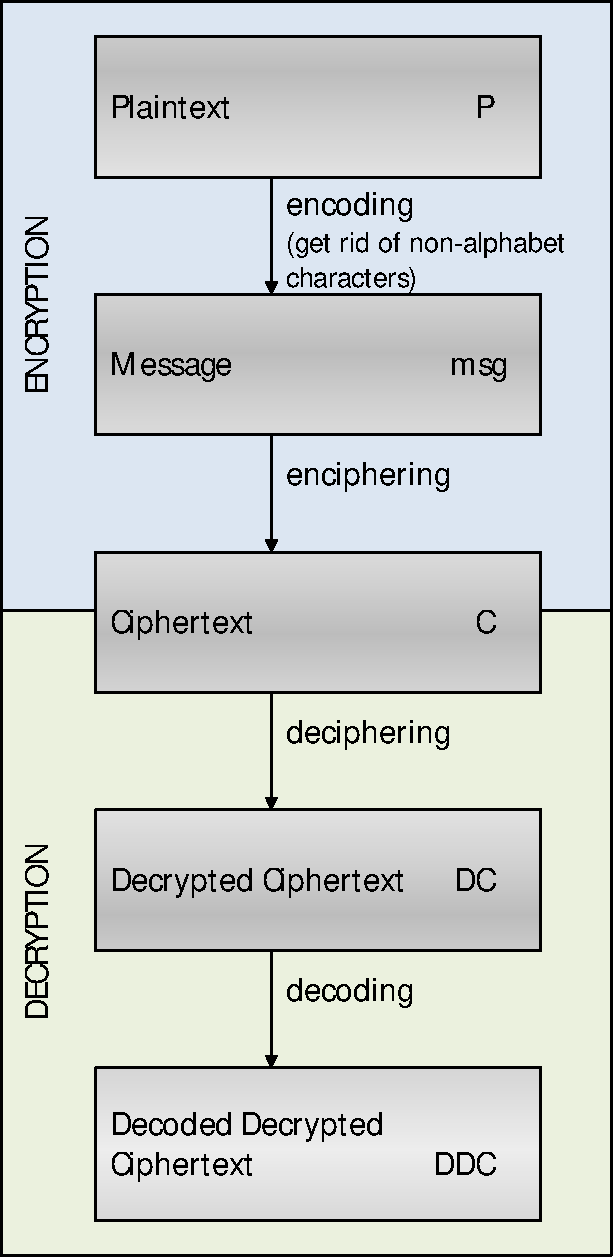
\includegraphics[scale=0.5]{figures/encryption-decryption-en}
\caption{Structure and naming convention of the Sage cipher code examples} 
\label{XXX}
\end{center}
\end{figure}



% ---------------------------------------------------------------------------
\newpage
\subsection{Transposition ciphers}

Tranposition ciphers are implemented in the Sage class
\begin{center}
\verb!sage.crypto.classical.TranspositionCryptosystem!
\end{center}
To construct and work with a transposition cipher, we first need to
determine the alphabet that contains the symbols used to build the space of our plaintext
and ciphertext. 
Typically, this alphabet will be the upper-case letters of the
English alphabet, which can be accessed via the function
\begin{center}
\verb!sage.monoids.string_monoid.AlphabeticStrings!
\end{center}
We then need to decide on the block length of a block permutation,
which is the length of the row vector to be used in the simple columns
transposition. This row vector is our key, and it specifies a permutation
of a plaintext.

The following first example of transposition ciphers has block length 14,
and the key is build in a way, that every letter
in the plaintext is shifted to the right by two characters, with wrap
around at the end of the block. That is the encryption process. The decryption process is
shifting each letter of the ciphertext to the left by $14 - 2 = 12$.

\begin{sagecode}
\begin{Verbatim}%
[fontsize=\footnotesize,fontshape=tt]
sage: # transposition cipher using a block length of 14
sage: T = TranspositionCryptosystem(AlphabeticStrings(), 14)
sage: # given plaintext
sage: P   = "a b c d e f g h i j k l m n"
sage: # encryption key
sage: key = [3, 4, 5, 6, 7, 8, 9, 10, 11, 12, 13, 14, 1, 2]
sage:
sage: # encode plaintext (get rid of non-alphabet chars, convert lower-case to upper-case)
sage: msg = T.encoding(P)
sage: # encrypt plaintext by shifting to the left by 2 letters (do it in two steps)
sage: E   = T(key)
sage: C   = E(msg); C
CDEFGHIJKLMNAB
sage:
sage: # decrypt ciphertext by shifting to the left by 12 letters
sage: keyInv = [13, 14, 1, 2, 3, 4, 5, 6, 7, 8, 9, 10, 11, 12]
sage: D   = T(keyInv)
sage: D(C)
ABCDEFGHIJKLMN
sage:
sage: # Representation of key and inverse key as permutations
sage: E
(1,3,5,7,9,11,13)(2,4,6,8,10,12,14)
sage: D
(1,13,11,9,7,5,3)(2,14,12,10,8,6,4)
\end{Verbatim}
\caption{Simple Transposition by shifting (key and inverse key explicitely given)}
\end{sagecode}

\newpage
The second example of transposition ciphers is also a simple shifting column transposition.
But now the code is a little bit more automated: The keys are generated from the shift parameter.

\begin{sagecode}
\begin{Verbatim}%
[fontsize=\footnotesize,fontshape=tt]
sage: # transposition cipher using a block length of 14, code more variable
sage: keylen = 14
sage: shift = 2
sage: A = AlphabeticStrings()
sage: T = TranspositionCryptosystem(A, keylen)
sage:
sage: # construct the plaintext string from the first 14 letters of the alphabet plus blanks
sage: # plaintext   = "A B C D E F G H I J K L M N"
sage: A.gens()
(A, B, C, D, E, F, G, H, I, J, K, L, M, N, O, P, Q, R, S, T, U, V, W, X, Y, Z)
sage: P=''
sage: for i in range(keylen): P=P + " " + str(A.gen(i))
....:
sage: P
' A B C D E F G H I J K L M N'
sage:
sage: # encryption key
sage: # key = [3, 4, 5, 6, 7, 8, 9, 10, 11, 12, 13, 14, 1, 2]
sage: key = [(i+shift).mod(keylen) + 1 for i in range(keylen)]; key
[3, 4, 5, 6, 7, 8, 9, 10, 11, 12, 13, 14, 1, 2]
sage:
sage: # encode plaintext (get rid of non-alphabet chars)
sage: msg = T.encoding(P)
sage: # encrypt plaintext by shifting to the left by 2 letters (do it in one step)
sage: C   = T.enciphering(key, msg); C
CDEFGHIJKLMNAB
sage:
sage: # decrypt ciphertext by shifting to the left by 12 letters
sage: # keyInv = [13, 14, 1, 2, 3, 4, 5, 6, 7, 8, 9, 10, 11, 12]
sage: shiftInv=keylen-shift;
sage: keyInv = [(i+shiftInv).mod(keylen) + 1 for i in range(keylen)]; keyInv
[13, 14, 1, 2, 3, 4, 5, 6, 7, 8, 9, 10, 11, 12]
sage: DC   = T.enciphering(keyInv, C); DC
ABCDEFGHIJKLMN
sage:
sage: # decryption using the "deciphering method with key" instead of "enciphering with keyInv" 
sage: # using the deciphering method requires to change the type of the variable key
sage: DC  = T.deciphering(T(key).key(), C); DC
ABCDEFGHIJKLMN
sage:
sage: # representation of key and inverse key as permutations
sage: T(key)
(1,3,5,7,9,11,13)(2,4,6,8,10,12,14)
sage: T(key).key()
(1,3,5,7,9,11,13)(2,4,6,8,10,12,14)
sage: T(keyInv)
(1,13,11,9,7,5,3)(2,14,12,10,8,6,4)
\end{Verbatim}
\caption{Simple Transposition by shifting (key and inverse key constructed with "range")}
\end{sagecode}

\newpage
In the third example of transposition ciphers we use an arbitrary permutation as key in the
encryption and decryption processes in order to scramble the characters within each
block (block length = number of columns in a simple column transposition).
If the block length is $n$, then the key must be a permutation on $n$ symbols.
The following example uses the method \verb!random_key()! of the class
\verb!TranspositionCryptosystem!. Each call to \verb!random_key()! produces a
different key. Note that therefore your results (key and ciphertext) may be different
from the following example.

\begin{sagecode}
\begin{Verbatim}%
[fontsize=\footnotesize,fontshape=tt]
sage: # Remark: Enciphering here requires, that the length of msg is a multiple of keylen
sage: keylen = 14   # length of key
sage: A = AlphabeticStrings()
sage: T = TranspositionCryptosystem(A, keylen); T
Transposition cryptosystem on Free alphabetic string monoid on A-Z of block length 14
sage:
sage: P = "a b c d e f g h i j k l m n o p q r s t u v w x y z a b"
sage: key = T.random_key(); key
(1,2,3,13,6,5,4,12,7)(11,14)
sage: msg = T.encoding(P); msg
ABCDEFGHIJKLMNOPQRSTUVWXYZAB
sage: C   = T.enciphering(key, msg); C
BCMLDEAHIJNGFKPQAZRSOVWXBUTY
sage: # decryption using the "deciphering method with key" instead of "enciphering with keyInv" 
ssage: DC  = T.deciphering(key, C); DC
ABCDEFGHIJKLMNOPQRSTUVWXYZAB
sage:
sage: # Just another way of decryption: Using "enciphering" with the inverse key
sage: keyInv = T.inverse_key(key); keyInv
(1,7,12,4,5,6,13,3,2)(11,14)
sage: DC     = T.enciphering(keyInv, C); DC
ABCDEFGHIJKLMNOPQRSTUVWXYZAB
sage:
sage: # Test correctness of decryption
sage: msg == DC
True
\end{Verbatim}
\caption{Simple Column Transposition with randomly generated (permutation) key}
\end{sagecode}


\newpage
The fourth example of transposition ciphers additionally shows the key space of a simple
column transpositon.

\begin{sagecode}
\begin{Verbatim}%
[fontsize=\footnotesize,fontshape=tt]
sage: keylen = 14   # length of key
sage: A = AlphabeticStrings()
sage: T = TranspositionCryptosystem(A, keylen); T
Transposition cryptosystem on Free alphabetic string monoid on A-Z of block length 14
sage: T.key_space()
Symmetric group of order 14! as a permutation group
sage: # Remark: The key space is not quite correct as also permutations shorter than keylen are counted.
sage:
sage: P = "a b c d e f g h i j k l m n o p q r s t u v w x y z a b"
sage: key = T.random_key(); key
(1,2,7)(3,9)(4,5,10,12,8,13,11)(6,14)
sage: msg = T.encoding(P); msg
ABCDEFGHIJKLMNOPQRSTUVWXYZAB
sage:
sage: # enciphering in one and in two steps
sage: C   = T.enciphering(key, msg); C
BGIEJNAMCLDHKFPUWSXBOAQZRVYT
sage:
sage: enc = T(key); enc.key()
(1,2,7)(3,9)(4,5,10,12,8,13,11)(6,14)
sage: C = enc(msg); C
BGIEJNAMCLDHKFPUWSXBOAQZRVYT
sage:
sage: # deciphering
sage: DC  = T.deciphering(key, C); DC
ABCDEFGHIJKLMNOPQRSTUVWXYZAB
\end{Verbatim}
\caption{Simple Column Transposition (showing the key\_space)}
\end{sagecode}



% ---------------------------------------------------------------------------
\newpage
\subsection{Substitution ciphers}

Substitution cryptosystems are implemented in Sage in the class
\begin{center}
\verb!sage.crypto.classical.SubstitutionCryptosystem!
\end{center}

\noindent The following code sample uses Sage to construct a substitution
cipher with a random key. A random key can be generated using the
method \verb!random_key()! of the class
\texttt{SubstitutionCryp\-to\-system}. Different keys determine different
substitution ciphers. So each call to \verb!random_key()! returns
different results.

\begin{sagecode}
\begin{Verbatim}%
[fontsize=\footnotesize,fontshape=tt]
sage: # plaintext/ciphertext alphabet
sage: A   = AlphabeticStrings()
sage: S   = SubstitutionCryptosystem(A)
sage:
sage: P   = "Substitute this with something else better."
sage: key = S.random_key(); key
INZDHFUXJPATQOYLKSWGVECMRB
sage:
sage: # method encoding can be called from A or from T
sage: msg = A.encoding(P); msg
SUBSTITUTETHISWITHSOMETHINGELSEBETTER
sage: C   = S.enciphering(key, msg); C
WVNWGJGVGHGXJWCJGXWYQHGXJOUHTWHNHGGHS
sage:
sage: #### We now decrypt the ciphertext to recover our plaintext.
sage:
sage: DC  = S.deciphering(key, C); DC
SUBSTITUTETHISWITHSOMETHINGELSEBETTER
sage: msg == DC
True
\end{Verbatim}
\caption{Monoalphabetic Substitution with randomly generated key}
\end{sagecode}



% ---------------------------------------------------------------------------
\newpage
\subsection{Caesar cipher}

The following example uses Sage to construct a Caesar
cipher.

\begin{sagecode}
\begin{Verbatim}%
[fontsize=\footnotesize,fontshape=tt]
sage: # plaintext/ciphertext alphabet
sage: A = AlphabeticStrings()
sage: P = "Shift the alphabet three positions to the right."
sage:
sage: # construct Caesar cipher
sage: S = SubstitutionCryptosystem(A)
sage: key = A([3, 4, 5, 6, 7, 8, 9, 10, 11, 12, 13, 14, 15, 16, 17, 18, 19, \
....:          20, 21, 22, 23, 24, 25, 0, 1, 2])
sage:
sage: # encrypt message
sage: msg     = A.encoding(P); msg
SHIFTTHEALPHABETTHREEPOSITIONSTOTHERIGHT
sage: encrypt = S(key); encrypt
DEFGHIJKLMNOPQRSTUVWXYZABC
sage: C       = encrypt(msg); C
VKLIWWKHDOSKDEHWWKUHHSRVLWLRQVWRWKHULJKW
sage:
sage: #### Next, we recover the plaintext.
sage:
sage: # decrypt message
sage: keyInv = A([23, 24, 25, 0, 1, 2, 3, 4, 5, 6, 7, 8, 9, 10, 11, 12, 13, \
....:             14, 15, 16, 17, 18, 19, 20, 21, 22])
sage: decrypt = S(keyInv); decrypt
XYZABCDEFGHIJKLMNOPQRSTUVW
sage: DC      = decrypt(C); DC
SHIFTTHEALPHABETTHREEPOSITIONSTOTHERIGHT
sage: msg == DC
True
\end{Verbatim}
\caption{Caesar (substitution by shifting the alphabet; key explicitely given, step-by-step approach)}
\end{sagecode}


\newpage
\noindent The second Caesar sample does the same, but the code is more sophisticated/automated/var\-i\-a\-ble.

\begin{sagecode}
\begin{Verbatim}%
[fontsize=\footnotesize,fontshape=tt]
sage: # plaintext/ciphertext alphabet
sage: A = AlphabeticStrings()
sage: keylen = len(A.gens()); keylen
26
sage: shift  = 3
sage: P = "Shift the alphabet three positions to the right."
sage:
sage: # construct Caesar cipher
sage: S = SubstitutionCryptosystem(A)
sage: S
Substitution cryptosystem on Free alphabetic string monoid on A-Z
sage: # key = A([3, 4, 5, 6, 7, 8, 9, 10, 11, 12, 13, 14, 15, 16, 17, 18, 19, \
sage: #          20, 21, 22, 23, 24, 25, 0, 1, 2])
sage: key = [(i+shift).mod(keylen) for i in range(keylen)];
sage: key = A(key); key
DEFGHIJKLMNOPQRSTUVWXYZABC
sage: len(key)
26
sage:
sage: # encrypt message
sage: msg     = A.encoding(P); msg
SHIFTTHEALPHABETTHREEPOSITIONSTOTHERIGHT
sage: C       = S.enciphering(key, msg); C
VKLIWWKHDOSKDEHWWKUHHSRVLWLRQVWRWKHULJKW
sage:
sage: #### Next, we recover the plaintext.
sage:
sage: # decrypt message
sage: # keyInv = A([23, 24, 25, 0, 1, 2, 3, 4, 5, 6, 7, 8, 9, 10, 11, 12, 13, \
sage: #             14, 15, 16, 17, 18, 19, 20, 21, 22])
sage: shiftInv=keylen-shift;
sage: keyInv = [(i+shiftInv).mod(keylen) for i in range(keylen)];
sage: keyInv = A(keyInv); keyInv
XYZABCDEFGHIJKLMNOPQRSTUVW
sage: DC     = S.enciphering(keyInv, C); DC
SHIFTTHEALPHABETTHREEPOSITIONSTOTHERIGHT
sage:
sage: # Just another way of decryption: Using "deciphering" with the key
sage: DC     = S.deciphering(key, C); DC
SHIFTTHEALPHABETTHREEPOSITIONSTOTHERIGHT
sage:
sage: msg == DC
True
\end{Verbatim}
\caption{Caesar (substitution by shifting the alphabet; substitution keys are generated)}
\end{sagecode}



% ---------------------------------------------------------------------------
\newpage
\subsection{Substitution with symbols}

In the following Sage example the symbols are from the binary number
system. A monoalphabetic substitution cipher with a binary alphabet has very little
security: Because the plaintext/ciphertext alphabet has only the two elements
0 and 1, there are only two keys possible: (0 1) and (1 0). Remark: In each key of a
substitution cipher all symbols of the alphabet have to appear once.

\begin{sagecode}
\begin{Verbatim}%
[fontsize=\footnotesize,fontshape=tt]
sage: # the plaintext/ciphertext alphabet
sage: A = BinaryStrings()
sage: # substitution cipher over the alphabet A; no keylen argument possible
sage: S = SubstitutionCryptosystem(A); S
Substitution cryptosystem on Free binary string monoid
sage: # to have a substitute for each symbol, key has always the length of the alphabet
sage: key = S.random_key(); key
10
sage: len(key)
2
sage: P = "Working with binary numbers."
sage: # encryption
sage: msg = A.encoding(P); msg
01010111011011110111001001101011011010010110111001100111001000000111011101101\
00101110100011010000010000001100010011010010110111001100001011100100111100100\
1000000110111001110101011011010110001001100101011100100111001100101110
sage: C   = S.enciphering(key, msg); C
10101000100100001000110110010100100101101001000110011000110111111000100010010\
11010001011100101111101111110011101100101101001000110011110100011011000011011\
0111111001000110001010100100101001110110011010100011011000110011010001
sage: # decryption
sage: DC  = S.deciphering(key, C); DC
01010111011011110111001001101011011010010110111001100111001000000111011101101\
00101110100011010000010000001100010011010010110111001100001011100100111100100\
1000000110111001110101011011010110001001100101011100100111001100101110
sage: msg == DC
True
\end{Verbatim}
\caption{Monoalphabetic substitution with a binary alphabet}
\end{sagecode}



\newpage
The second sample of a monoalphabetic substitution with symbols uses  a larger alphabet
as plaintext/ciphertext space as the first sample. Here the hexadecimal number system
is used as substitution alphabet.

\begin{sagecode}
\begin{Verbatim}%
[fontsize=\footnotesize,fontshape=tt]
sage: A = HexadecimalStrings()
sage: S = SubstitutionCryptosystem(A)
sage: key = S.random_key(); key
2b56a4e701c98df3
sage: len(key)
16
sage: # Number of possible keys
sage: factorial(len(key))
20922789888000
sage: P   = "Working with a larger alphabet."
sage:
sage: msg = A.encoding(P); msg
576f726b696e6720776974682061206c617267657220616c7068616265742e
sage: C   = S.enciphering(key, msg); C
47e375e9e1efe75277e17ae052eb52e8eb75e7e47552ebe872e0ebe5e47a5f
sage: DC  = S.deciphering(key, C); DC
576f726b696e6720776974682061206c617267657220616c7068616265742e
sage: msg == DC
True
sage:
sage: # Conversion hex back to ASCII:
sage: # - AlphabeticStrings() and HexadecimalStrings() don't have according methods.
sage: # - So we used Python:
sage: #   - repr(DC) converts the StringMonoidElement DC to a string
sage: #     still containing hex symbols;
sage: #   - binascii.a2b_hex converts this hex string to an ascii string.
sage: import binascii
sage: DDC = binascii.a2b_hex(repr(DC)); DDC
'Working with a larger alphabet.'
sage:
sage: P == DDC
True
\end{Verbatim}
\caption{Monoalphabetic substitution with a hexadecimal alphabet (and decoding in Py\-thon)}
\end{sagecode}



% ---------------------------------------------------------------------------
\newpage
\subsection{Vigen{\`e}re cipher}

The Vigen{\`e}re cipher is implemented in the Sage class
\begin{center}
\verb!sage.crypto.classical.VigenereCryptosystem!
\end{center}

\noindent For our ciphertext/plaintext space, we can work with the upper-case
letters of the English alphabet, the binary number system, the
octal number system, or the hexadecimal number system. Here is an
example using the class \verb!AlphabeticStrings!, which implements
the English capital letters.

\begin{sagecode}
\begin{Verbatim}%
[fontsize=\footnotesize,fontshape=tt]
sage: # construct Vigenere cipher
sage: keylen = 14
sage: A = AlphabeticStrings()
sage: V = VigenereCryptosystem(A, keylen); V
Vigenere cryptosystem on Free alphabetic string monoid on A-Z of period 14
sage:
sage: # alternative: given key: key = A('ABCDEFGHIJKLMN'); key
sage: key = V.random_key(); key
WSSSEEGVVAARUD
sage: len(key)
14
sage:
sage: # encoding
sage: P = "The Vigenere cipher is polyalphabetic."
sage: len(P)
38
sage: msg = V.encoding(P); msg     # alternative: msg = A.encoding(P); msg
THEVIGENERECIPHERISPOLYALPHABETIC
sage:
sage: # encryption [2 alternative ways (in two steps or in one): both work]
sage: # encrypt = V(key); encrypt
sage: # C = encrypt(msg); C
sage: C   = V.enciphering(key, msg); C
PZWNMKKIZRETCSDWJAWTUGTALGBDXWLAG
sage:
sage: # decryption
sage: DC  = V.deciphering(key, C); DC
THEVIGENERECIPHERISPOLYALPHABETIC
sage: msg == DC
True
\end{Verbatim}
\caption{Vigen{\`e}re cipher}
\end{sagecode}




% ---------------------------------------------------------------------------
\newpage
\subsection{Hill cipher}

The Hill~\cite{pp:Hill1929,pp:Hill1931} or matrix cipher is more
mathematically sophisticated than other ciphers mentioned in this
chapter. The encryption/decryption key of this cipher is an invertible
square matrix, and the plaintext/ciphertext is processed also as a matrix.
The encryption and decryption processes use matrix operations. The Hill
cipher is implemented in the Sage class
\begin{center}
\verb!sage.crypto.classical.HillCryptosystem!
\end{center}

In the following example our plaintext/ciphertext space is the
capital letters of the English alphabet. In the Hill cipher, each
letter of this alphabet is assigned a unique integer modulo 26.

\begin{sagecode}
\begin{Verbatim}%
[fontsize=\footnotesize,fontshape=tt]
sage: # construct a Hill cipher
sage: keylen = 19    # keylen = 3  # Alternative key length with non-random small key
sage: A = AlphabeticStrings()
sage: H = HillCryptosystem(A, keylen); H
Hill cryptosystem on Free alphabetic string monoid on A-Z of block length 19
sage:
sage: # To create key non-randomly, HKS is necessary [even H.key_space() is not enough].
sage: # HKS = H.key_space()
sage: # key = HKS([[1,0,1],[0,1,1],[2,2,3]]); key
sage:
sage: # Random key creation
sage: key = H.random_key(); key
[10  7  5  2  0  6 10 23 15  7 17 19 18  2  9 12  0 10 11]
[23  1  1 10  4  9 21  1 25 22 19  8 17 22 15  8 12 25 22]
[ 4 12 16 15  1 12 24  5  9 13  5 15  8 21 23 24 22 20  6]
[ 5 11  6  7  3 12  8  9 21 20  9  4 16 18 10  3  2 23 18]
[ 8 22 14 14 20 13 21 19  3 13  2 11 13 23  9 25 25  6  8]
[24 25  8 24  7 18  3 20  6 11 25  5  6 19  7 24  2  4 10]
[15 25 11  1  4  7 11 24 20  2 18  4  9  8 12 19 24  0 12]
[14  6  2  9 11 20 13  4 10 11  4 23 14 22 14 16  9 12 18]
[12 10 21  5 21 15 16 17 19 20  1  1 15  5  0  2 23  4 14]
[21 15 15 16 15 20  4 10 25  7 15  4  7 12 24  9 19 10  6]
[25 15  2  3 17 23 21 16  8 18 23  4 22 11 15 19  6  0 15]
[14 23  9  3 18 15 10 18  7  5 12 23 11  9 22 21 20  4 14]
[ 3  6  8 13 20 16 11  1 13 10  4 21 25 15 12  3  0 11 18]
[21 25 14  6 11  3 21  0 19 17  5  8  5  4  9  2 23 19 15]
[ 8 11  9 11 20 15  6  1  3 18 18 22 16 17  6  3 15 11  2]
[21 15  5 22  2  9  0  4 22 10  2 10 19 19 17 19  1 21  4]
[ 7 17  9  2 15  5 14  3  6  9 12 12 22 15  8  4 21 14 19]
[19 14 24 19  7  5 22 22 13 14  7 18 17 19 25  2  1 23  6]
[ 2  6 14 22 17  7 23  6 22  7 13 20  0 14 23 17  6  1 12]
sage:
sage: # encoding and encryption
sage: P = "Hill or matrix cipher uses matrix operations."
sage: len(P)
45
sage: # implementation requires: Length of msg is a multiple of matrix dimension (block_length)
sage: msg = H.encoding(P); msg
HILLORMATRIXCIPHERUSESMATRIXOPERATIONS
sage: len(msg)
38
sage:
sage: # encryption
sage: C  = H.enciphering(key, msg); C
CRWCKPRVYXNBRZTNZCTQWFWSDWBCHABGMNEHVP
sage:
sage: # decryption
sage: DC  = H.deciphering(key, C); DC
HILLORMATRIXCIPHERUSESMATRIXOPERATIONS
sage: msg == DC
True
sage:
sage: # alternative decryption using inverse matrix
sage: keyInv = H.inverse_key(key); keyInv
[ 6 23  1 23  3 12 17 22  6 16 22 14 18  3  1 10 21 16 20]
[18 23 15 25 24 23  7  4 10  7 21  7  9  0 13 22  5  5 23]
...
[10 11 12  6 11 17 13  9 19 16 14 24  4  8  5 16 18 20  1]
[19 16 16 21  1 19  7 12  3 18  1 17  7 10 24 21  7 16 11]
sage: DC     = H.enciphering(keyInv, C); DC
HILLORMATRIXCIPHERUSESMATRIXOPERATIONS
\end{Verbatim}
\caption{Hill cipher}
\end{sagecode}







% --------------------------------------------------------------------------
\newpage
\begin{thebibliography}{99999}
\addcontentsline{toc}{section}{Bibliography}

\bibitem[ACA2002]{pp:ACA2002} \index{ACA 2002}
   American Cryptogram Association, \\
   {\em Length and Standards for all ACA Ciphers}, \\
   2002.\\
   \href{http://www.cryptogram.org/cdb/aca.info/aca.and.you/chap08.html#}
   {\texttt{http://www.cryptogram.org/cdb/aca.info/aca.and.you/chap08.html\#}}

\bibitem[Bauer1995]{pp:Bauer1995} \index{Bauer 1995}
    Friedrich L. Bauer, \\
    {\em Entzifferte Geheimnisse}, Springer, 1995.

\bibitem[Bauer2000]{pp:Bauer2000} \index{Bauer 2000}
    Friedrich L. Bauer, \\
    {\em Decrypted Secrets}, Springer 1997, 2nd edition 2000.
	
\bibitem[Crowley2000]{pp:Crowley2000} \index{Crowley 2000}
   Paul Crowley, \\
   {\em Mirdek: A card cipher inspired by ``Solitaire''}, \\
   2000.\\
   \href{http://www.ciphergoth.org/crypto/mirdek/}
   {\texttt{http://www.ciphergoth.org/crypto/mirdek/}}

\bibitem[DA1999]{pp:DA1999} \index{DA 1999}
   Data encryption page of the ThinkQuest Team 27158 for ThinkQuest 1999 \\
   (no update since 1999, no search possibility), \\
   1999.\\
   \href{http://library.thinkquest.org/27158/}
   {\texttt{http://library.thinkquest.org/27158/}}

\bibitem[Goebel2003]{pp:Goebel2003} \index{Goebel 2003}
   Greg Goebel, \\
   {\em Codes, Ciphers and Codebreaking}, \\
   2003.\\
   \href{http://www.vectorsite.net/ttcode.htm}
   {\texttt{http://www.vectorsite.net/ttcode.htm}}

\bibitem[Hill1929]{pp:Hill1929} \index{Hill 1929}
   Lester S. Hill,\\
   ``Cryptography in an Algebraic Alphabet,''
   \emph{The American Mathematical Monthly}, 36(6):306--312, 1929.

\bibitem[Hill1931]{pp:Hill1931} \index{Hill 1931}
   Lester S. Hill,\\
   ``Concerning Certain Linear Transformation Apparatus of Cryptography,''
   \emph{The American Mathematical Monthly}, 38(3):135--154, 1931.

\bibitem[Nichols1996]{pp:Nichols1996} \index{Nichols 1996} 
    Randall K. Nichols, \\
    {\em Classical Cryptography Course, Volume 1 and 2}, \\
    Aegean Park Press 1996;
    or in 12 lessons online at \\
    \href{http://www.fortunecity.com/skyscraper/coding/379/lesson1.htm}
    {\texttt{http://www.fortunecity.com/skyscraper/coding/379/lesson1.htm}}

\bibitem[Savard1999]{pp:Savard1999} \index{Savard 1999}
	John J. G. Savard, \\
	{\em A Cryptographic Compendium}, \\
	1999.\\
	\href{http://www.hypermaths.org/quadibloc/crypto/jscrypt.htm}
	{\texttt{http://www.hypermaths.org/quadibloc/crypto/jscrypt.htm}}
	
\bibitem[Schmeh2004]{pp:Schmeh2004}  \index{Schmeh 2004}
        Klaus Schmeh, \\
        {\em Die Welt der geheimen Zeichen. Die faszinierende Geschichte
        der Verschl\"usselung},\\ 
        W3L Verlag Bochum, 1. Auflage 2004.

\bibitem[Schmeh2007]{pp:Schmeh2007}  \index{Schmeh 2007}
        Klaus Schmeh, \\
        {\em Codeknacker gegen Codemacher. Die faszinierende Geschichte der Verschl\"usselung.},\\ 
        W3L Verlag Bochum, 2. Auflage 2007.\\
	This is most current among the books dealing in a comprehensive manner with the history of cryptology. It contains a small collection of solved and unsolved crypto riddles.

\bibitem[Schneier1999]{pp:Schneier1999}
	Bruce Schneier, \\
	{\em The Solitaire Encryption Algorithm}, \\
	version 1.2, 1999.\\
	\href{http://www.schneier.com/solitaire.html}
	{\texttt{http://www.schneier.com/solitaire.html}}

\bibitem[Singh2001]{pp:Singh2001} \index{Singh 2001}
	Simon Singh, \\
	{\em Geheime Botschaften. Die Kunst der Verschl\"usselung von der 
        Antike bis in die Zeiten des Internet}, \\
	dtv, 2001.

\bibitem[ThinkQuest1999]{pp:ThinkQuest1999} \index{ThinkQuest 1999}
	ThinkQuest Team 27158, \\
	{\em Data Encryption}, \\
	1999.\\
	\href{http://library.thinkquest.org/27158/}
	{\texttt{http://library.thinkquest.org/27158/} }

\end{thebibliography}









% Local Variables:
% TeX-master: "../script-en.tex"
% End:

